\section{Quality vs output length}
\label{app:quality}

DG degrades gracefully against a \emph{time} budget
and catastrophically against an \emph{output-length} budget. At
$L{=}128$ the AR model retains \arFOneTwentyEight{} F1 and
\arValidTwentyEight\% schema validity, while DG falls
to \dgFOneTwentyEight{} and \dgValidTwentyEight\%. Which budget an
application faces decides which architecture is safer;
Figure~\ref{fig:quality} traces both curves.

\begin{figure}[ht!]
\centering
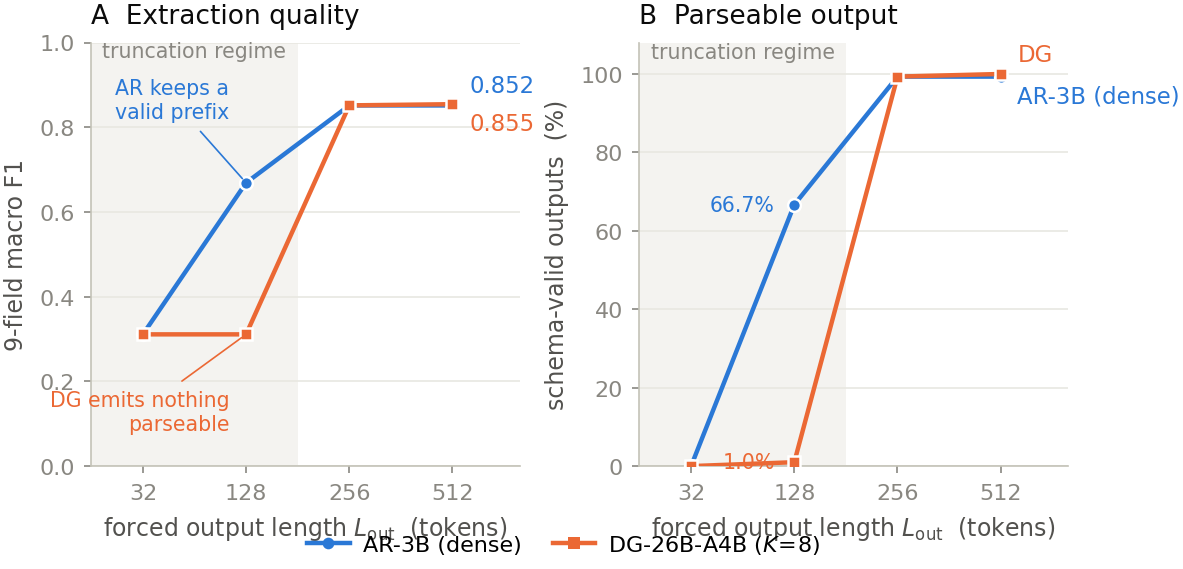
\includegraphics[width=\linewidth]{figures/fig5_quality_vs_length.png}
\caption{Quality and schema validity vs forced output length (BGL,
$n{=}300$; AR arm is dense AR-3B). \textbf{A:} DG's 9-field F1 rises
with $L$ and plateaus, while AR-3B is flat from $L{=}256$ to $L{=}512$
because first-object-wins parsing discards the rambled continuation.
\textbf{B:} schema validity is the sharper split, at $L{=}128$ DG
returns a valid record \dgValidTwentyEight\% of the time against
AR-3B's \arValidTwentyEight\%, because a canvas truncated below its
length is not a complete JSON object. This is the hard floor on DG's
completeness guarantee.}
\label{fig:quality}
\end{figure}
